\documentclass[a4paper, 12pt]{article}
\usepackage[a4paper,top=1.5cm, bottom=1.5cm, left=1cm, right=1cm]{geometry}
\usepackage[utf8]{inputenc}
\usepackage{mathtext}
\usepackage{amsmath}
\usepackage{amsfonts}
\usepackage[english, russian]{babel}
\usepackage{indentfirst}
\usepackage{longtable}
\usepackage{graphicx}
\graphicspath{{pictures/}}
\DeclareGraphicsExtensions{.pdf,.png,.jpg}
\usepackage{natbib}
\usepackage{hyperref}
\usepackage{emoji}
\babelfont{rm}{Droid Serif}
\babelfont{sf}{Droid Sans}
\renewcommand{\baselinestretch}{1.3}

\title{1.3.1. Определение модуля Юнга на основе исследования деформаций растяжения и изгиба}
\author{Платонов Егор Б04-301}
\date{\today}

\begin{document}

\maketitle

\textbf{Цель работы:} экспериментально получить зависимость между напряжением и деформацией для одностороннего сжатия, вычислить модуль Юнга.

\textbf{В работе используются:} в первой части - прибор Лермантова, проволока
    из исследуемого материала,
     зрительная трубка со шкалой,
    набор грузов, микрометр, рулетка;  во второй части - стойка для изгибания балки, индикатор для
    измерения величин прогиба,
набор исследуемых стержней, грузы, линейка, штангенциркуль.

\section{Определение модуля Юнга по измерениям растяжения проволоки}
    \subsection{Теоретические сведения}
    Растяжение проволоки соответствует напряженному состоянию вдоль одной оси, которое описывается формулой:
\begin{equation}
    \frac{F}{S} = E \frac{\Delta l}{l}
    \label{lermantov}
\end{equation}
Измерения производятся на установке Лермантова.
    Направим зрительную трубку на зеркальце.
    Выведем формулу для расчета растяжения длины проволоки по показаниям шкалы
    прибора (см. рис. 1).
    Так как мы считаем проволоку слабо растяжимой, справедлива оценка $\Delta l \ll r$, где
    $r$ -- длина рычага. С учетом этого, угол наклона зеркальца к горизонтали можно
    найти как $\alpha = \Delta l/r$. С другой стороны, из соображений геометрической оптики
    угол $\alpha$ можно найти как угол между продолжениями соответствующих лучей:
    \begin{equation}
        \alpha = \frac{n}{2h},
    \end{equation}
    где $n$ -- показания шкалы, $h$ -- расстояние от шкалы до
    зеркальца.
    \par Таким образом, удлинение проволоки можно выразить как:
    \begin{equation}
        \Delta l = n\frac{r}{2h}
        \label{dlina}
    \end{equation}

    Отсюда формулу (1) можно переписать как
    \begin{equation}
        F = \frac{ESr}{2lh}n
    \end{equation}

\begin{figure}[h]
        \centering
        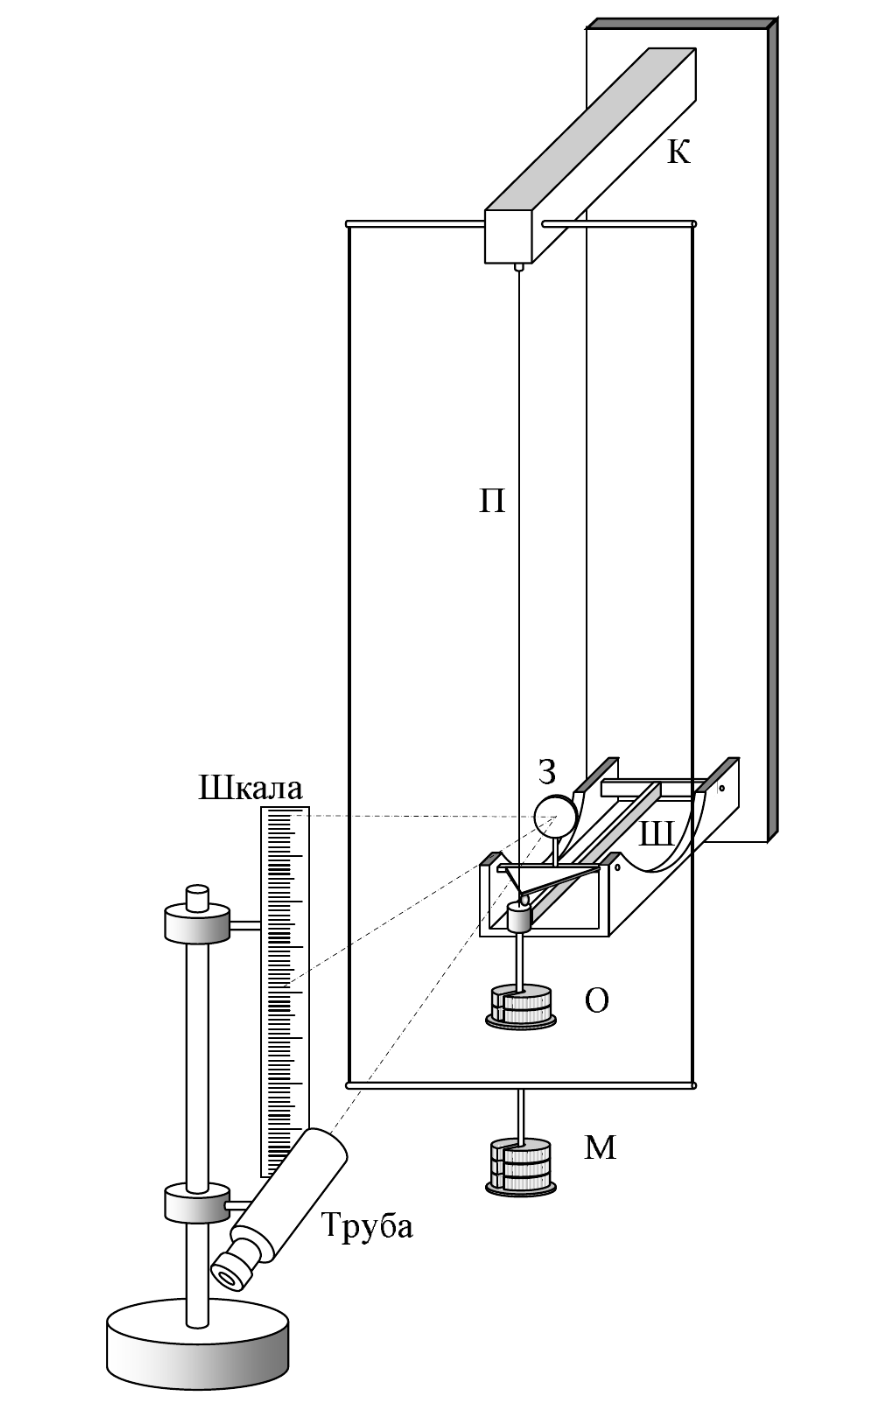
\includegraphics[scale = 0.5]{lermantov.png}
        \caption{Прибор Лермантова}
    \end{figure}

\section{Измерения и обработка результатов}

Диаметр проволоки $d = 0,51$ мм, по формуле $S=\frac{\pi d^2}{4}$ найдена площадь поперечного сечения $S = 0,204$ мм $^2$

Длина проволоки $l=(174,2 \pm 0,1)$ см, $\varepsilon_l = 0,06\%$

Расстояние от зеркала до шкалы $h = (143,6 \pm 0,1)$ см, $\varepsilon_h = 0,07\%$

Длина рычага $r = 20$ мм

Предельная нагрузка найдена по формуле $F_{max} = 0.3\sigma_{max} S = 55,8$ Н, где $\sigma_{max} = 900$ Н/мм$^2$

Зависимость $\Delta l$ от F, при возрастании нагрузки, представлена в таблице 1, зависимость $\Delta l$ от F, при убывании нагрузки, представлена в таблице 2.

\begin{table}[ht]
 \centering
    \parbox{.4 \textwidth}{
        \centering
        \begin{tabular}{|l|l|l|l|}
        \hline
            $m$, г & $F$, Н & $n\uparrow$, см & $\Delta l\uparrow$, см \\ \hline
            455,3 & 4,47 & 13,1 & 0,91 \\ \hline
            700,5 & 6,87 & 15,4 & 1,07 \\ \hline
            945,3 & 9,27 & 17,2 & 1,2 \\ \hline
            1190,6 & 11,68 & 19,2 & 1,34 \\ \hline
            1435,5 & 14,08 & 21,1 & 1,47 \\ \hline
            1681 & 16,49 & 23 & 1,6 \\ \hline
            1926,8 & 18,9 & 24,4 & 1,7 \\ \hline
            2172,5 & 21,31 & 26,1 & 1,82 \\ \hline
            2418,4 & 23,72 & 27,7 & 1,93 \\ \hline
            2663,7 & 26,13 & 29,2 & 2,03 \\ \hline
        \end{tabular}
        \caption{Зависимость $\Delta l$ от F, при возрастании нагрузки}
        \label{tab:1}
    }
    \hfill
    \parbox{.5 \textwidth}{
        \centering
        \begin{tabular}{|l|l|l|l|}
        \hline
            $m$, г & $F$, Н & $n\downarrow$, см & $\Delta l\downarrow$, см \\ \hline
            455,3 & 4,47 & 13,1 & 0,91 \\ \hline
            700,5 & 6,87 & 15,5 & 1,08 \\ \hline
            945,3 & 9,27 & 17,4 & 1,21 \\ \hline
            1190,6 & 11,68 & 19,3 & 1,34 \\ \hline
            1435,5 & 14,08 & 21 & 1,46 \\ \hline
            1681 & 16,49 & 22,8 & 1,59 \\ \hline
            1926,8 & 18,9 & 24,6 & 1,71 \\ \hline
            2172,5 & 21,31 & 26,2 & 1,82 \\ \hline
            2418,4 & 23,72 & 27,7 & 1,93 \\ \hline
            2663,7 & 26,13 & 29,2 & 2,03 \\ \hline
        \end{tabular}
        \caption{Зависимость $\Delta l$ от F, при убывании нагрузки}
        \label{tab:2}
    }
 \end{table}
Зависимости изображены графически на рисунке 2.
\begin{figure}[h]
    \centering
    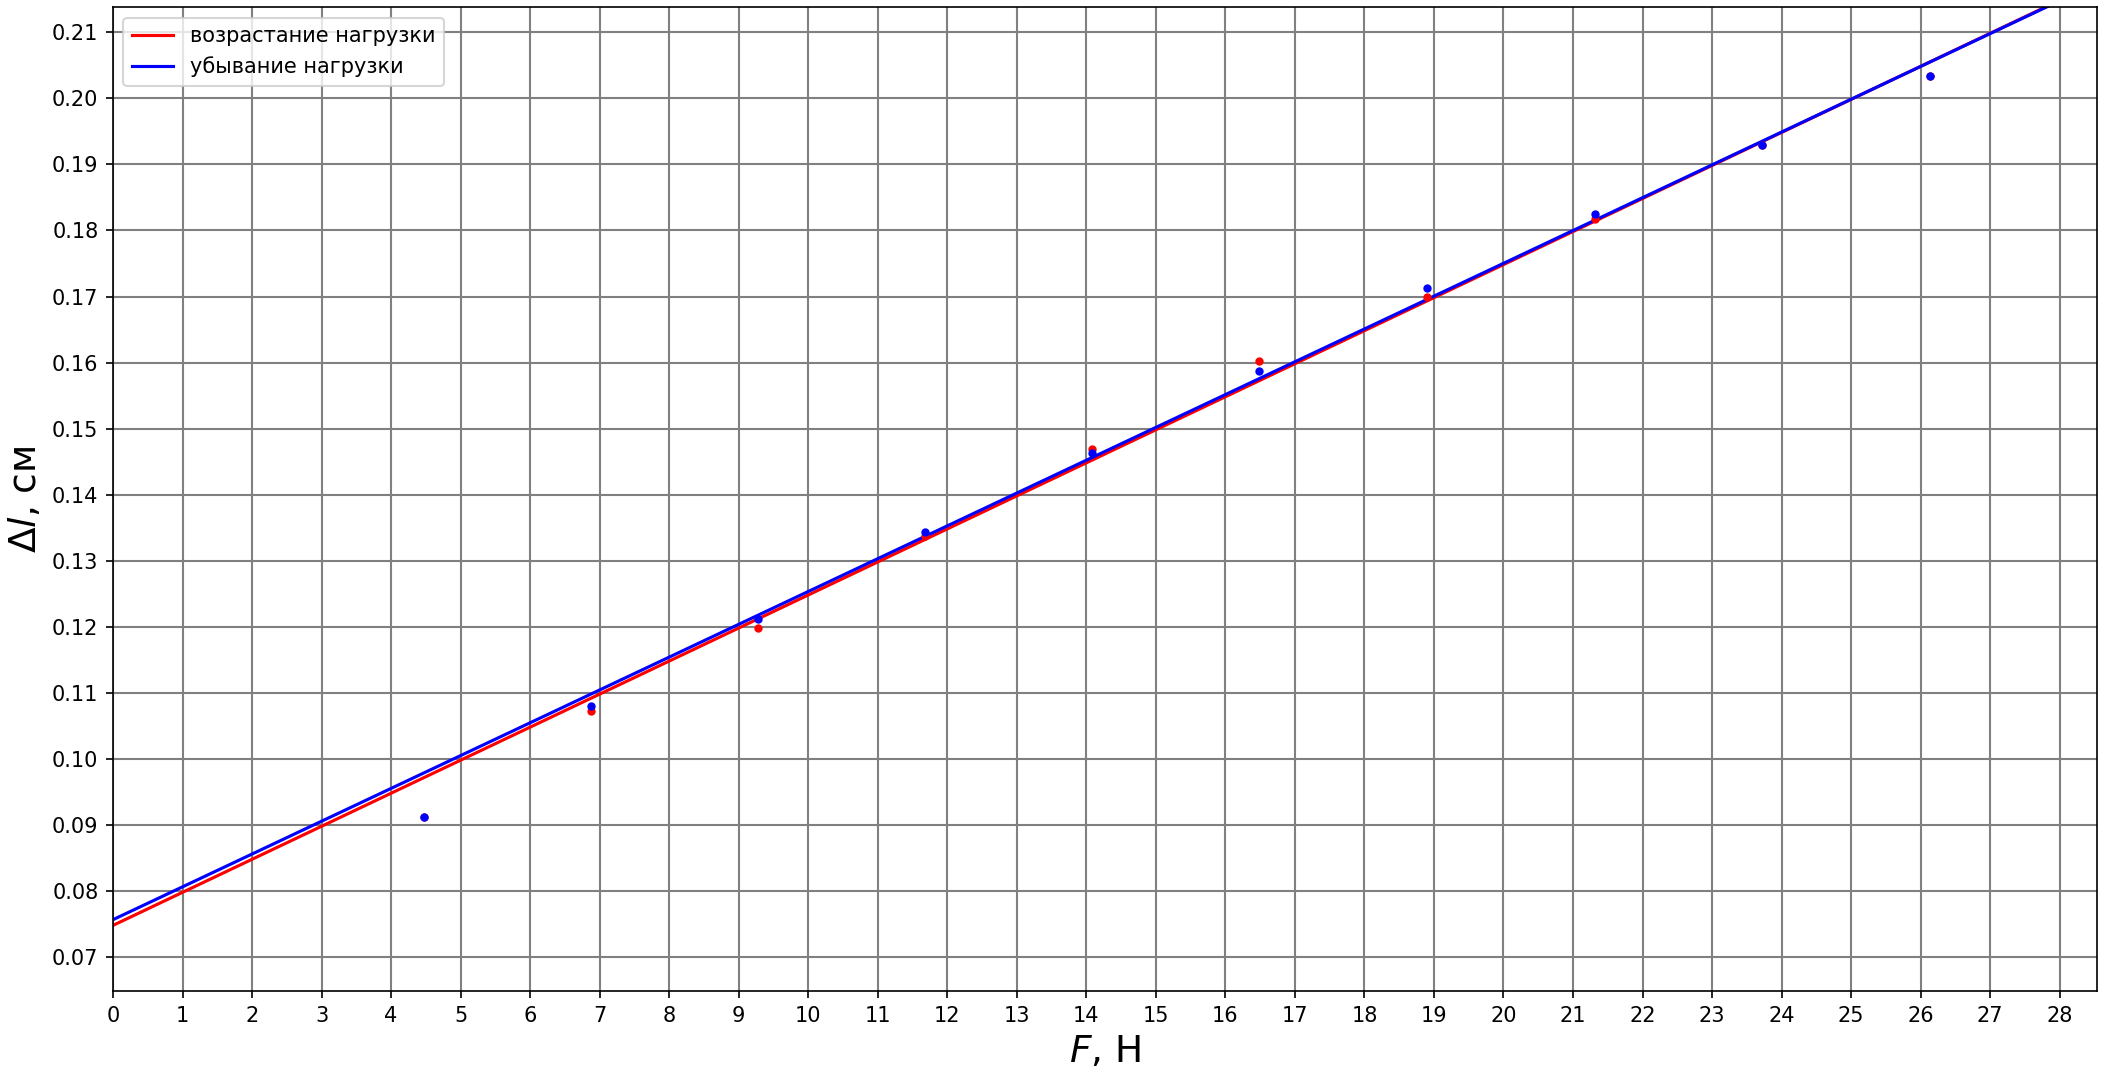
\includegraphics[scale = 0.5]{plot.png}
    \caption{Зависимость $\Delta l(F)$}
    \label{fig:enter-label}
\end{figure}
 В линейной аппроксимации не учитывалась первая точка, так как при небольшой нагрузке проволока выпрямляется, а растяжение (линейный участок) начинается уже при большем весе.

По МНК найдены коэффициенты наклона $k_1 \approx k_2$ = 0,005 $\frac{\text{см}}{\text{Н}}$ = 0,00005 $\frac{\text{м}}{\text{Н}}$. При подсчете систематической погрешности учтено, что относительные погрешности величин примерно одинаковые, в формуле используется $\Delta l$, ближайшее к среднему ($\varepsilon_n = 0,2 \%$).

\[ \sigma_k^{\text{случ}} = \frac{1}{\sqrt{N - 2}}\sqrt{\frac{\langle {\Delta l}^2 \rangle -\langle {\Delta l} \rangle^2}{
    \langle F^2 \rangle - \langle F \rangle^2} - k^2}\]

\[ \sigma_k^{\text{сист}} = k\frac{\sigma_{\Delta l}}{\Delta l} = k\sqrt{\varepsilon_n^2+\varepsilon_l^2+\varepsilon_h^2}\]

\[ \sigma_{k2} \approx \sigma_{k1} = \sqrt{\sigma_k^{{\text{сист}}^2}+\sigma_k^{{\text{случ}}^2}} = 0,00008 \text{ }\frac{\text{см}}{\text{Н}}\]

\[ \varepsilon_k = \frac{\sigma_k}{k} = 1,6 \%\]
    
Если $k = \frac{\Delta l}{F}$, то из формулы (1) следует, что
\[ E = \frac{l}{Sk} = \frac{4l}{\pi d^2k} = 170,5 \text{ ГПа}\]

\[ \varepsilon_E = \sqrt{\varepsilon_k^2+\varepsilon_l^2} = 1,6 \%\]
Помимо модуля Юнга $E$ вычислена и жесткость проволоки $k'$:
\[k' = \frac{SE}{l} = \frac{\pi d^2 E}{4l} = 20 \frac{\text{кН}}{\text{м}}\]

\section{Вывод}
В работе была подтверждена линейная зависимость удлиннения от приложенной силы, найден модуль Юнга проволоки $ E = 170,5 \text{ ГПа}$ с точностью 1,6\%. Если сравнивать с табличными данными, то такое значение модуля Юнга ближе всего к платине (168 ГПа), что вряд ли соответствует действительности. Скорее всего проволока сделана из стали (200-210 Гпа) или из железа (190-200 ГПа), с некоторыми примесями, понижающими значение модуля Юнга.

\end{document}
